\begin{frame}
\frametitle{Decrypting files without access to a tool}
\begin{block}{Problem Statement}
    \begin{itemize}
        \item Faced with a large number of encrypted files.
        \item Encryption uses a custom implementation.
        \item No available command-line tool for decryption.
        \item The key and/or IV has been recovered.
        \item Debugging and manual decryption of each file is time-consuming and inefficient.
    \end{itemize}
\end{block}
\end{frame}

\begin{frame}
\frametitle{Decrypting Files Without Access to a Tool}
\begin{block}{Traditional Approach}
\begin{itemize}
    \item Write a loader program to execute the code.
    \item Read the code into a buffer.
    \item Cast the buffer to a function pointer.
    \item Execute the function pointer.
    \item \textbf{Challenges:}
    \begin{itemize}
        \item Buffers are often protected against code execution.
        \item Requires fiddling with \texttt{mmap} and \texttt{mprotect}.
        \item The code might include malicious instructions that went unidentified.
        \item The decryptor may be designed for another CPU architecture (e.g., MIPS, RISC-V).
    \end{itemize}
\end{itemize}
\end{block}
\end{frame}

\begin{frame}
    \frametitle{Decrypting Files Without Access to a Tool}
    \begin{itemize}
        \item The Unicorn Engine\footnote{\url{https://www.unicorn-engine.org/}} is a CPU emulator based on QEMU.
        \item Supports multiple architectures:
        \begin{itemize}
            \item ARM, ARM64 (ARMv8), m68k, MIPS, PowerPC, RISC-V, S390x (SystemZ), SPARC, TriCore, and x86 (including x86\_64).
        \end{itemize}
        \item Provides bindings for various programming languages:
        \begin{itemize}
            \item Pharo, Crystal, Clojure, Visual Basic, Perl, Rust, Haskell, Ruby, Python, Java, Go, D, Lua, JavaScript, .NET, Delphi/Pascal, and MSVC.
        \end{itemize}
        \item Offers hooking capabilities for:
        \begin{itemize}
            \item \textbf{Memory access}, \textbf{executed instructions}, and \textbf{interrupts}.
        \end{itemize}
        \item Thread-safe\footnote{Multithreading is often used as an anti-debugging technique.}
        \item Works without modifying code (e.g., no need to insert instructions such as \texttt{INT3} or \texttt{0xCC}).
    \end{itemize}
\end{frame}

\begin{frame}[fragile]
\frametitle{Building Unicorn Engine}
\begin{block}{Prerequisites}
    Install the required tools:
    \begin{itemize}
        \item \texttt{cmake}
        \item \texttt{pkg-config}
    \end{itemize}
    \textbf{Command:}
    \begin{verbatim}
sudo apt install cmake pkg-config
    \end{verbatim}
\end{block}

\end{frame}

\begin{frame}[fragile]
\frametitle{Building Unicorn Engine}

\begin{block}{Build Steps}
    Follow these steps to build Unicorn:
    \begin{enumerate}
        \item Create and navigate to the build directory:
        \begin{verbatim}
mkdir build; cd build
        \end{verbatim}
        \item Run \texttt{cmake} with the release build type:
        \begin{verbatim}
cmake .. -DCMAKE_BUILD\_TYPE=Release
        \end{verbatim}
        \item Compile the project and install it:
        \begin{verbatim}
make & make install
        \end{verbatim}

    \end{enumerate}
\end{block}
\end{frame}


% Define code style
\lstset{
    basicstyle=\ttfamily\scriptsize, % Font style and size
    keywordstyle=\color{blue},       % Color for keywords
    commentstyle=\color{green!60!black}, % Color for comments
    stringstyle=\color{red},         % Color for strings
    numbers=left,                    % Line numbers on the left
    numberstyle=\tiny,               % Line number font size
    frame=single,                    % Frame around the code
    breaklines=true,                 % Line breaking
    showstringspaces=false           % Hide spaces in strings
}


\begin{frame}[fragile]
\frametitle{XOR Cipher Example in C 1/2}
\begin{lstlisting}[language=C]
#include <stdio.h>
#include <string.h>
// Function to encrypt/decrypt a string using XOR cipher
void xor_cipher(char *data, char key) {
    for (int i = 0; i < strlen(data); i++) {
        data[i] ^= key; // XOR each character with the key
    }
}
\end{lstlisting}
\end{frame}

\begin{frame}[fragile]
\frametitle{XOR Cipher Example in C 2/2}
\begin{lstlisting}[language=C]
int main() {
    char data[] = "Hello, World!";  // Message to encrypt
    char key = 'K';                // Encryption key

    printf("Original: %s\n", data);

    // Encrypt the data
    xor_cipher(data, key);
    printf("Encrypted: %s\n", data);

    // Decrypt the data
    xor_cipher(data, key);  // Apply XOR again with the same key to decrypt
    printf("Decrypted: %s\n", data);

    return 0;
}
\end{lstlisting}

\begin{lstlisting}{language=bash}
    gcc -o sample sample.c
\end{lstlisting}
\end{frame}

\begin{frame}
\frametitle{Determining Base Address}
In Ghidra, click on \textbf{Window} and then select \textbf{Memory Map}.
\vspace{1cm}
\centering
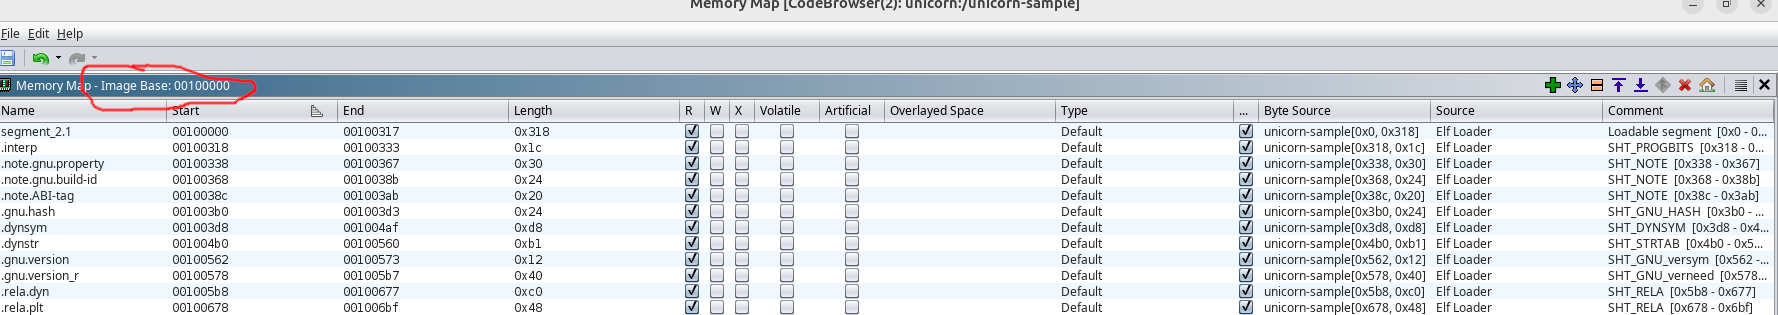
\includegraphics[scale=0.3]{img/base.png}
\end{frame}

\begin{frame}
    \frametitle{Determining the Start Address of the Function}
    \begin{itemize}
        \item \textbf{Challenge:} Identify the function or code block responsible for encryption.
        \item \textbf{Approach:} Look for functions containing numerous arithmetic and bitwise operations:
        \begin{itemize}
            \item Arithmetic operations: \texttt{ADD}, \texttt{SUB}, \texttt{MUL}, \texttt{DIV}.
            \item Bitwise operations: \texttt{XOR}, \texttt{SHR}, \texttt{SHL}.
        \end{itemize}
        \item Check for these operations grouped in blocks or loops.
    \end{itemize}
    \centering
    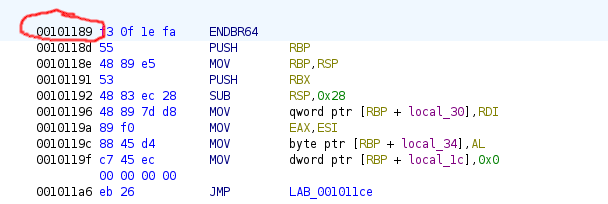
\includegraphics[scale=0.5]{img/start.png}
\end{frame}

\begin{frame}
    \frametitle{Determining the End of a Function}
    \begin{itemize}
        \item Functions often end with the \textbf{RET} instruction.
    \end{itemize}
    \vspace{1cm}
    \centering
    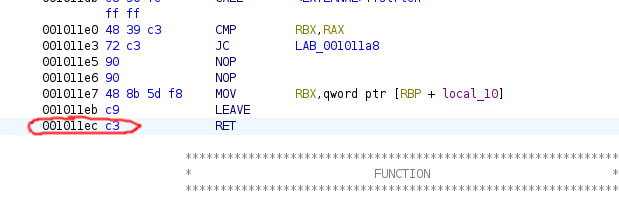
\includegraphics[scale=0.5]{img/end.png}
\end{frame}


\begin{frame}[fragile]
\frametitle{Python Code Example: Hooking in Unicorn Engine}
\begin{lstlisting}[language=Python, caption={Hooking Example with Unicorn Engine}]
from unicorn import *
from unicorn.x86_const import *

import struct

def hook_mem_access(uc, access, address, size, value, user_data):
    print(f"[*] Memory access: {access:x} at 0x{address:x}, data size = {size}, data value = 0x{value:x}")

def hook_code(uc, address, size, user_data):
    print(f"[*] Current RIP: {address:x}, instruction size = {size}")
\end{lstlisting}

\begin{itemize}
    \item Create a virtual environment and install the Python bindings.
    \item Import the necessary methods.
    \item Set up the hooking functions.
\end{itemize}

\end{frame}


\begin{frame}[fragile]
\frametitle{Python Code Example: Configuring the Engine}
\begin{lstlisting}[language=Python, caption={Unicorn Engine Example with Hooks}]
with open("sample", "rb") as f:
    binary = f.read()

ADDRESS = 0x1000000

uc = Uc(UC_ARCH_X86, UC_MODE_64)
uc.hook_add(UC_HOOK_MEM_WRITE, hook_mem_access)
uc.hook_add(UC_HOOK_MEM_READ, hook_mem_access)
uc.hook_add(UC_HOOK_CODE, hook_code, None, ADDRESS + 0x1189, ADDRESS + 0x12AC)
uc.mem_map(ADDRESS, 2 * 1024 * 1024)  # 2 MB
uc.mem_write(ADDRESS, binary)
\end{lstlisting}

\begin{itemize}
	\item Define the CPU architecture (line 6)
	\item Install the hooks (line 7 to 9)
	\item Configure memory layout (line 10)
	\item Load the ELF file (line 11)
\end{itemize}
\end{frame}

\begin{frame}[fragile]
\frametitle{Function Parameter Passing}
\begin{lstlisting}[language=Python, caption={Unicorn Engine Example: Setting Arguments}]
input_str = b".''$gk$9'/j"
input_key = 75 # 'K'  

# Write the input string to memory
uc.mem_write(ADDRESS + 0x4000, input_str)  # Address where input_str is stored (binary 16K, string at 17K)

# Set up registers
uc.reg_write(UC_X86_REG_RDI, ADDRESS + 0x4000)  # Set the first argument (address of the string)
uc.reg_write(UC_X86_REG_RSI, input_key)        # Set the second argument (offset)
uc.reg_write(UC_X86_REG_RSP, ADDRESS + 0x6000) # Set the stack (RSP)
\end{lstlisting}

Pay attention to the operating system's calling convention.
\end{frame}



\begin{frame}[fragile]
\frametitle{Python Code Example: Emulating with Unicorn}
\begin{lstlisting}[language=Python, caption={Unicorn Engine Emulation Example}]
try:
    # Start emulation from the specified range
    uc.emu_start(ADDRESS + 0x1189, ADDRESS + 0x11EC)  # Start and end addresses recovered from Ghidra

    # Read the result from memory and decode it
    result = uc.mem_read(ADDRESS + 0x4000, len(input_str)).decode("utf-8")
    print(f"Encoded string: {result}")

except UcError as e:
    # Handle errors during emulation
    print(f"Unicorn error: {e}")
\end{lstlisting}

\end{frame}

\begin{frame}[fragile]
\frametitle{Unicorn Engine Trouble Shooting}
\begin{minipage}{0.5\textwidth}
\begin{lstlisting}[basicstyle=\ttfamily\scriptsize,numbers=left, numberstyle=\tiny]
[*] Current RIP: 1001189, instruction size = 4
[*] Current RIP: 100118d, instruction size = 1
[*] Memory access: 11 at 0x1005ff8, data size = 8, data value = 0x0
[*] Current RIP: 100118e, instruction size = 3
[*] Current RIP: 1001191, instruction size = 1
[*] Memory access: 11 at 0x1005ff0, data size = 8, data value = 0x0
[*] Current RIP: 1001192, instruction size = 4
[*] Current RIP: 1001196, instruction size = 4
[*] Memory access: 11 at 0x1005fd0, data size = 8, data value = 0x1004000
\end{lstlisting}
\end{minipage}%
\hfill
\begin{minipage}{0.4\textwidth}
\centering
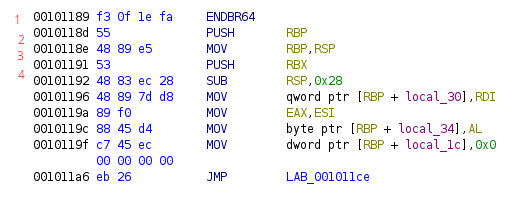
\includegraphics[scale=0.4]{img/block.png}
\end{minipage}
\end{frame}
